This chapter details the methodology adopted for evaluating Large Language Models (LLMs) in the context of Automated Program Repair (APR) using Python code. It describes the experimental setup, including the use of the Pytracebugs dataset, the prompt engineering strategies, and the suite of evaluation metrics designed to assess both syntactic and semantic correctness of model-generated repairs. The chapter also explains the implementation details, such as model execution, configuration of generation parameters, and the error handling and monitoring mechanisms employed to ensure reliable and reproducible results. The goal is to provide a clear and concise account of the procedures and tools used, enabling transparent and repeatable experimentation.
This chapter details the methodology adopted for evaluating Large Language Models (LLMs) in the context of Automated Program Repair (APR) using Python code. It describes the experimental setup, including the use of the Pytracebugs dataset, the prompt engineering strategies, and the suite of evaluation metrics designed to assess both syntactic and semantic correctness of model-generated repairs. The chapter also explains the implementation details, such as model execution and configurations.


\section{Dataset and datapreparation}

\subsection{Pytracebugs}
The experiment uses the Pytracebugs dataset \cite{Pytracebugs}, which contains Python source codes from GitHub repositories at the granularity of function snippets and their corresponding Traceback errors; see the example below.


\begin{figure}[h!]
    \centering
    \caption{An example of a single data point from the Pytracebugs dataset.}
    \label{fig:dataset-example}

    % (a) The Buggy Code
    \begin{lstlisting}[
        language=Python,
        frame=single,
        basicstyle=\ttfamily\small,
        caption={a) Buggy Code Snippet (\texttt{before\_merge})},
        belowcaptionskip=-0.5em % Adjust spacing
        ]
def noise(self, value):
  self.noise_covar.initialize(value)
    \end{lstlisting}

    % (b) The Traceback Error
    \begin{lstlisting}[
        frame=single,
        basicstyle=\ttfamily\small,
        caption={b) Traceback Error (\texttt{full\_traceback})},
        belowcaptionskip=-0.5em % Adjust spacing
        ]
import gpytorch
gl = gpytorch.likelihoods.GaussianLikelihood()
gl.initialize(noise=1)
Traceback (most recent call last):
File ""<stdin>"", line 1, in <module>
File "".../gpytorch/gpytorch/module.py"", line 89, in initialize
setattr(self, name, val)
File ""../lib/python3.6/site-packages/torch/nn/modules/module.py"", line 579, in __setattr__
object.__setattr__(self, name, value)
File "".../gpytorch/gpytorch/likelihoods/gaussian_likelihood.py"", line 63, in noise
self.noise_covar.initialize(value)
TypeError: initialize() takes 1 positional argument but 2 were given
    \end{lstlisting}

    % (c) The Fixed Code
    \begin{lstlisting}[
        language=Python,
        frame=single,
        basicstyle=\ttfamily\small,
        caption={c) Fixed Code Snippet (\texttt{after\_merge})}
        ]
def noise(self, value):
  self.noise_covar.initialize(noise=value)
    \end{lstlisting}
\end{figure}

\begin{figure}[h!]
    \centering
    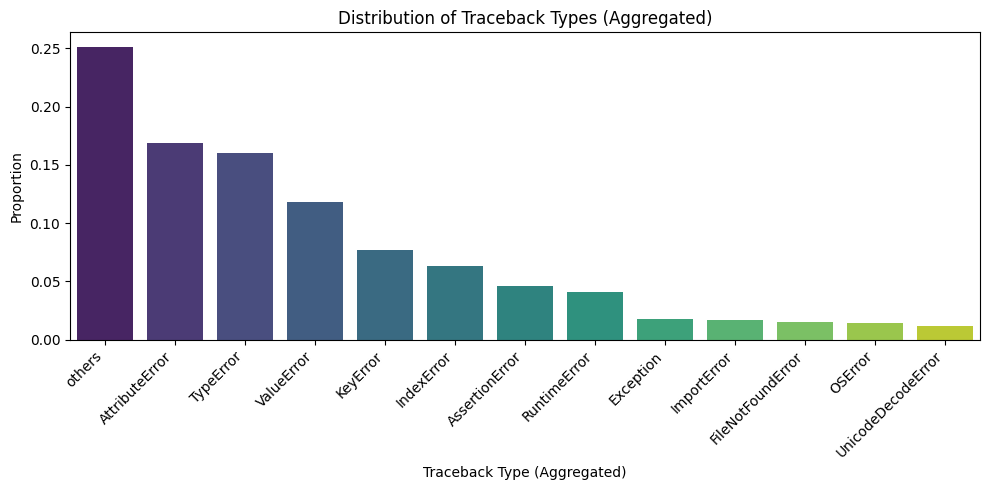
\includegraphics[width=0.7\textwidth]{Cap2/dataset-traceback-type.png}
    \caption{Distribution of Error Types in the dataset - Less than 1\% relevant are consolidated into 'others' category.}
    \label{fig:dataset-traceback-types}
\end{figure}

Most frequent traceback errors can be found in Figure \ref{fig:dataset-traceback-types}, with the most frequent ones being Atribute Error and TypeError with $16.84\%$ and $16\%$ of the values respectivelly. Also, there is a significant amount of erros that appear less than $1\%$ of the time, and were aggregated into the 'Others' Category.

%TODO: Adicionar exemplos de trabalhos publicados que utilizam como referencia o dataset proposto.
Some published works that use this dataset aim to study problems such as Vulnerability Detection \cite{zhao2024coding} and fault localization \cite{kulkarni2024graph}.

\subsection{LLM Models}
The model selection for this experiment was guided by three criteria: (1) representation of different architectural approaches, (2) availability through OpenRouter API, and (3) cost-effectiveness for large-scale experimentation. Four models were selected to provide a balanced comparison across these dimensions.

Two open-source models specialized in code generation were included: Qwen 2.5 Coder 32B (instruct) \cite{hui2024qwen25codertechnicalreport} and Codestral 2501 \cite{Codestral_202501}. These models represent the current state-of-the-art in open-source code generation, with Qwen 2.5 Coder 32B achieving competitive performance on coding benchmarks while maintaining significantly lower computational requirements compared to larger models.

Two closed-source models were selected for comparison: Claude 3.5 Sonnet and GPT-4o. These models represent the current frontier of general-purpose language models and provide a baseline for evaluating whether specialized code models offer advantages over general-purpose architectures in automated program repair tasks.

The selection of exactly four models balances statistical power requirements with computational feasibility. While larger model sets could provide more comprehensive comparisons, the chosen sample size allows for robust statistical analysis while maintaining manageable experimental costs.

% TODO: adicionar referencias que confirmem que os modelos estão dentre os modelos de estado da arte no período. Benchmarks

%TODO: encontrar referências que comprovem que modelos especialistas tem vantagens específicas.

%TODO: Pesquisar referencias de statistical power LLM experiments. para justificar por que 4 modelos são suficientes.

%TODO: Argumentar por que outros modelos não foram escolhidos.

% For the first experiment, four models were chosen. Two of these are open-source models specialized in code generation, considered state-of-the-art in this category: Qwen 2.5 coder 32b (instruct) \cite{hui2024qwen25codertechnicalreport} and Codestral 2501 \cite{Codestral_202501}. Additionally, two state-of-the-art, commonly used closed-source models of a relatively similar size were selected: Claude $3.5$ Sonnet and GPT $4o$ Model.

Although these models are all similarly competitive in structured benchmarks, they differ considerably in terms of usage cost. For reference, the token cost for each selected model is shown in Table \ref{tab:model-tokens}.
\begin{table}[h!]
\centering
\caption{Token usage price per model.}
\label{tab:model-tokens}
\begin{tabular}{|l|c|c|}
\hline
\textbf{Model} & \textbf{Input Tokens (1M)} & \textbf{Output Tokens (1M)} \\ \hline
Claude Sonnet 3.5 & \$3.0 & \$15.0 \\ \hline
Gpt 4o & \$2.5 & \$10 \\ \hline
Codestral 2501 & \$0.3 & \$0.9 \\ \hline
Qwen 2.5 Coder 32B Instruct & \$0.05 & \$0.20 \\ \hline
\end{tabular}
\end{table}
% todo addicionar gemini flas
%TODO melhorar a argumentação desses modelos
% Falar do tamanho dos modelos e da comparabilidade deles. Exibir ranking. Existem muitos, portanto qualquer escolha tem uma arbitrariedade. Não vamos todos no hugging faces.

% TODO trazer artigos que divulgam esses modelos.

\section{Experimental Design}
\subsection{Prompt variations}

To test the model's sensitivity to the prompt's instructions, all prompts were formatted 
using a consistent template, shown in Listing \ref{lst:prompt-template}. This structure ensures 
that each model receives the context—buggy code and traceback error—in a clear, delimited 
format, and is explicitly asked to return only the corrected code.

% The 'figure' environment helps manage the placement and captioning of the listing.
\begin{figure}[h!]
% This is the crucial line that starts the code block.
% The formatting options are placed in the square brackets.
\begin{lstlisting}[
    caption={The general template used for all prompts.},
    label={lst:prompt-template},
    basicstyle=\ttfamily\small,
    frame=single,
    breaklines=true
]
{{ instruction_prompt }}

### BUGGY CODE:
{{ buggy_code }}

### ERROR:
{{ traceback_error }}

### RETURN ONLY THE CORRECTED CODE BELOW:

IMPORTANT: Return ONLY the corrected/requested code. Do not include any explanations, comments about the changes, or other text. Just return the pure code.

\end{lstlisting} % This line correctly ends the code block.
\end{figure}
% It clearly isolates the variable you are testing.
\begin{table}[h!]
\centering
\caption{Instruction variations for the \texttt{instruction\_prompt} variable.}
\label{tab:prompt-instructions}
\begin{tabular}{|l|p{0.55\textwidth}|p{0.15\textwidth}|}
\hline
\textbf{Prompt ID} & \textbf{Instruction Text} & \textbf{System Prompt} \\ \hline
P1 (Baseline) & You are a helpful assistant that corrects the code based on the traceback error. & False. \\\hline
P2 (Style-aware) & You are a helpful assistant that corrects the code based on the traceback error. You must respect the original code structure and the original code style. & False. \\ \hline
P3 (System Prompt) & You are a helpful assistant that corrects the code based on the traceback error. & True. \\ \hline
\end{tabular}
\end{table}
The core of the experiment lies in the variation of the \texttt{instruction\_prompt} placeholder and the addition of system prompt. 
We designed three distinct instructions, which we will refer to as P1 (Baseline) and P2 (Style-aware) and P3 (System Prompt), 
to evaluate the impact of a more detailed directive. The specific text for each instruction 
is detailed in Table \ref{tab:prompt-instructions}.

\subsubsection{Justification of Prompt Variations}
The selection of these three specific prompt variations was driven by theoretical considerations in prompt engineering and their relevance to automated program repair tasks. Each variation was designed to test a distinct hypothesis about how LLMs process and respond to different types of instructions.

\textbf{P1 (Baseline):} This prompt serves as the experimental control, providing minimal instruction to establish a baseline performance level. The simplicity of this prompt allows us to measure the inherent capability of each model without additional constraints, serving as a reference point for evaluating the effectiveness of more specific instructions. This approach follows the principle of establishing a null hypothesis in experimental design, where we can assess whether additional prompt complexity actually improves performance.

\textbf{P2 (Style-aware):} The style-aware prompt introduces explicit constraints about preserving code structure and style, addressing a critical concern in automated program repair. Previous research has shown that LLMs can generate syntactically correct but stylistically inconsistent code \cite{wang2025functionalcorrectnessinvestigatingcoding}, which may reduce code maintainability and increase cognitive load for developers. By explicitly instructing the model to respect original code structure and style, we test whether such constraints lead to more maintainable and contextually appropriate patches. This variation is particularly relevant for production environments where code consistency is paramount.

\textbf{P3 (System Prompt):} This variation tests the hypothesis that system-level instructions, which have higher precedence in the API message hierarchy, can provide more consistent and reliable behavior than instruction-level prompts. System prompts are designed to establish global behavioral patterns and are processed differently by the model's architecture. By moving the instruction to the system level, we investigate whether this architectural difference results in more deterministic and consistent code generation, which is crucial for automated repair systems that require reliability and reproducibility.

The systematic variation between these three conditions allows us to isolate the effects of instruction specificity (P1 vs. P2) and instruction placement (P2 vs. P3), providing insights into both the content and delivery mechanisms that influence LLM performance in code repair tasks.

\subsubsection{Prompt Roles in API requests}
\begin{itemize}
    \item \textbf{System prompt:} It is an initialization message that sets global behavior for the model across a conversation or a request. It encodes policies, personas, output formatting, and safety constraints. In most APIs, it has a higher precedence than user instructions. The typical contents usually are guardrails, style registers, and output contracts (e.g., ``always return strict python code'').
    \item \textbf{Instruction prompt:} describes a specific task to perform. it is scoped to the current step/turn and it is subordinate to the system message when they conflict. Typical contents usually are task descriptions, inputs, and desired outputs for the tasks.
\end{itemize}

At inference, the API concatenates messages (System -> Developer -> user->assistant history) into a single token sequence. "Priority" is learned behavior, not a hard rule.

\subsection{Experiment tracking}
The experimental design employed a systematic sampling approach to ensure statistical validity while maintaining computational feasibility. A random sample of 300 buggy code instances was selected from the Pytracebugs dataset for each model-prompt combination, resulting in a total of 4 × 300 × 3 = 3600 experimental trials.

To estimate the statistical power for our sample size, we approximated the paired comparison using Cohen's $d$ and a normal distribution. For $n=300$ paired instances per condition, a family-wise significance level $\alpha_\text{family}=0.01$ with $K=4$ comparisons yields an individual threshold
\[
\alpha_\text{indiv} = \frac{\alpha_\text{family}}{K} = 0.0025,
\]
corresponding to
\[
z_{1-\alpha_\text{indiv}/2} \approx 3.09.
\]
Assuming a small-to-medium effect size of $d \approx 0.3$, the non-central parameter is
\[
\text{ncp} = d \cdot \sqrt{n} \approx 5.196.
\]
The resulting approximate power is
\[
\text{Power} \approx 1 - \Phi(z_{1-\alpha_\text{indiv}/2} - \text{ncp}) \approx 0.982,
\]
indicating that the chosen sample size is sufficient to detect meaningful effects while keeping computational cost reasonable.


% TODO: descrever escolha randomica de experimento e tamanho de amostra que resulte em Significancia estatística necessária para tirarmos conclusões a respeito dos resultados.

To ensure statistical rigor in our evaluation, we conducted a power analysis to verify that our sample size of 300 paired instances per condition was adequate. We used a family-wise significance threshold of $\alpha = 0.01$ for confirmatory comparisons, applying corrections for multiple testing across models. With this setup, 300 samples provide high power (approximately 0.98) to detect effects of small-to-medium size (Cohen's $d \approx 0.3$), which matches the expected effect sizes in this task. Detecting very small effects ($d \approx 0.2$) would require larger samples, but our chosen size balances computational cost and statistical validity, ensuring that meaningful differences can be detected with strong confidence.

For each response, the following evaluation metrics were computed: AST similarity, AST-normalized score, CodeBLEU, N-gram overlap, weighted N-gram match, syntax correctness, and dataflow preservation. Each metric was evaluated against both the original buggy code and the ground truth correction to provide comprehensive performance assessment.

\section{Evaluation Method}
\label{sec:evaluation-method}

The evaluation framework employs multiple complementary metrics to assess the quality of generated code repairs across different dimensions: structural similarity, semantic preservation, and syntactic correctness. This multi-faceted approach ensures comprehensive assessment of LLM performance in automated program repair tasks.

\subsection{Structural Similarity Metrics}

\subsubsection{AST Score}
The Abstract Syntax Tree (AST) score measures the structural similarity between the generated repair code and the ground truth correction by comparing their parsed trees. This metric is particularly relevant for our type of problem since it captures the fundamental program structure independently of formatting, variable names, or comment variations.

The AST score is computed by:
\begin{enumerate}
    \item Parsing both the generated code and ground truth into their respective AST representations;
    \item Computing the tree edit distance using the Zhang-Shasha algorithm \cite{zhang1989simple};
    \item Normalizing the distance by the maximum tree size to obtain a similarity score in the range [0,1];
\end{enumerate}

A score of 1.0 indicates perfect structural similarity, while 0.0 represents completely different program structures. This metric is sensitive to control flow changes, function structure modifications, and overall program architecture, making it essential for evaluating whether the LLM has preserved the intended program logic.

\subsubsection{AST Normalized Score}
The AST normalized score addresses a fundamental limitation of the raw AST score by normalizing identifiers and constants to focus purely on structural similarity. This metric is particularly valuable in automated program repair as it distinguishes between structural changes and mere naming variations, which are often irrelevant to the actual repair quality.
% TODO: Confirm this
The normalization process involves:
\begin{enumerate}
    \item Parsing both the generated code and ground truth into AST representations
    \item Applying a normalization transformation that:
        \begin{itemize}
            \item Replaces variable names with normalized identifiers (\texttt{\_var\_1}, \texttt{\_var\_2}, etc.)
            \item Replaces function names with normalized identifiers (\texttt{\_func\_1}, \texttt{\_func\_2}, etc.)
            \item Replaces class names with normalized identifiers (\texttt{\_class\_1}, \texttt{\_class\_2}, etc.)
            \item Replaces literal constants with a placeholder (\texttt{\_const\_})
        \end{itemize}
    \item Computing similarity between the normalized AST representations using sequence matching
\end{enumerate}

This approach is crucial for automated program repair evaluation because it focuses on the essential structural logic rather than superficial naming differences. For example, a repair that changes variable names from \texttt{user\_input} to \texttt{input\_data} would receive a perfect normalized AST score, while maintaining the same structural integrity. This metric is particularly valuable for identifying whether LLMs are generating repairs that preserve the intended program logic and control flow, regardless of identifier choices.

To illustrate the difference between AST and AST normalized representations, consider the following example of a Python function:

\begin{figure}[h!]
\centering
\begin{minipage}{0.46\textwidth}
\centering
\textbf{Original AST}
\begin{lstlisting}[basicstyle=\ttfamily\tiny, frame=single, breaklines=true]
Module(
  body=[
  FunctionDef(
    name='check_status',
    args=arguments(
      posonlyargs=[],
      args=[
        arg(arg='monster'),
        arg(arg='status_name')],
      kwonlyargs=[],
      kw_defaults=[],
      defaults=[]),
    body=[
      Return(
        value=Call(
          func=Name(id='any', ctx=Load()),
          args=[
            GeneratorExp(
              elt=Name(id='t', ctx=Load()),
              generators=[
                comprehension(
                  target=Name(id='t', ctx=Store()),
                  iter=Attribute(
                    value=Name(id='monster', ctx=Load()),
                    attr='status',
                    ctx=Load()),
                  ifs=[
                    Compare(
                      left=Attribute(
                        value=Name(id='t', ctx=Load()),
                        attr='name',
                        ctx=Load()),
                      ops=[
                        Eq()],
                      comparators=[
                        Name(id='status_name', ctx=Load())])],
                  is_async=0)])],
          keywords=[]))],
    decorator_list=[])],
  type_ignores=[])
\end{lstlisting}
\end{minipage}
\hfill
\begin{minipage}{0.50\textwidth}
\centering
\textbf{AST Normalized}
\begin{lstlisting}[basicstyle=\ttfamily\tiny, frame=single, breaklines=true]
Module(
  body=[
  FunctionDef(
    name='_func_1',
    args=arguments(
      posonlyargs=[],
      args=[
        arg(arg='monster'),
        arg(arg='status_name')],
      kwonlyargs=[],
      kw_defaults=[],
      defaults=[]),
    body=[
      Return(
        value=Call(
          func=Name(id='_var_1', ctx=Load()),
          args=[
            GeneratorExp(
              elt=Name(id='_var_2', ctx=Load()),
              generators=[
                comprehension(
                  target=Name(id='_var_2', ctx=Store()),
                  iter=Attribute(
                    value=Name(id='_var_4', ctx=Load()),
                    attr='status',
                    ctx=Load()),
                  ifs=[
                    Compare(
                      left=Attribute(
                        value=Name(id='_var_2', ctx=Load()),
                        attr='name',
                        ctx=Load()),
                      ops=[
                        Eq()],
                      comparators=[
                        Name(id='_var_6', ctx=Load())])],
                  is_async=0)])],
          keywords=[]))],
    decorator_list=[])],
  type_ignores=[])
\end{lstlisting}
\end{minipage}
\caption{Side-by-side comparison of AST and AST normalized representations for the same Python function. The normalized version replaces specific identifiers with generic placeholders (\texttt{\_func\_1}, \texttt{\_var\_1}, etc.) while preserving the structural logic.}
\label{fig:ast-comparison}
\end{figure}

As shown in Figure \ref{fig:ast-comparison}, the AST normalized representation replaces specific identifiers like \texttt{check\_status}, \texttt{any}, \texttt{monster}, \texttt{status\_name}, and \texttt{t} with generic placeholders (\texttt{\_func\_1}, \texttt{\_var\_1}, \texttt{\_var\_4}, \texttt{\_var\_6}, and \texttt{\_var\_2} respectively). This normalization allows the metric to focus purely on structural similarity, ignoring naming variations that are irrelevant to the actual repair quality.

The AST normalized score provides a more robust assessment of repair quality by isolating structural changes from naming conventions, making it essential for evaluating whether the core program architecture and logic flow have been preserved in the generated repair.

\subsection{Dataflow Preservation}

\subsubsection{Dataflow}

\subsection{Semantic Similarity Metrics}
\subsubsection{Workflow N-gram}

\subsubsection{CodeBLEU}


\section{Implementation Details}
\subsection{Model Execution}
\label{sec:implementation-details}

All API calls to the proprietary models (GPT-4o and Claude 3.5 Sonnet) and the open-source models (Qwen 2.5 and Codestral) were managed through the \textbf{OpenRouter} API aggregation service. This approach was chosen to ensure a consistent and reproducible experimental setup across all models from a single interface.

The specific model identifiers used on the platform are listed below. To ensure that the results were as deterministic as possible and to facilitate a fair comparison, the generation parameters were kept constant for all API calls: a \textbf{temperature of 0} and a \textbf{top\_p of 1.0} were used. All experiments were conducted in \textbf{July 2025}.
\subsection{Retry Logic and Monitoring}

%todo: explicar melhor como gerenciamos os requests da api.
Our project implements a robust error handling mechanism, to ensure reliable operation. We captured and logged all API failures, and employed an exception handling strategy. So when individual API requests failed, then the system gracefully handles these exceptions by storing error messages in a result array, alowing the experiment to continue processing subsequent samples while maintaining a complete audit trail of all failures.

Also, the system utilizes structured logging to track metric calculation anomalies, specifically for CodeBLEU. We captured detailed information about dataflow extraction problems that could affect evaluation accuracy. 
% \begin{itemize}
%     \item \texttt{openai/gpt-4o}
%     \item \texttt{anthropic/claude-3.5-sonnet}
%     \item \texttt{qwen/qwen-2.5-coder-32b-instruct} 
%     \item \texttt{mistralai/codestral-2501}
% \end{itemize}
